\newpage
\section{Автоматическая имитация возраста}

Методы имитации возраста подразделяются на две категории. Методы первой категории используют знания, полученные из анатомических исследований кожи и мимики лица, чтобы затем интерпретировать определенные параметры лица как критерии возраста. Методы второй категории используют алгоритмы машинного обучения для того, чтобы автоматически вычленить те изменения в параметрах лица, что соответствуют старению. 

\subsection{Методы, основанные на анатомии лица}

Измеряя такие параметры лица, как высота лба, размер носа, положение уголков губ у женщин от 25 до 65 Pitanguy et al. \cite{pitanguy1} \cite{pitanguy2} установили строгую корреляцию между этими параметрами и возрастом. В результате была построена модель имитации возраста, основанная на изменении пропорций и искривлении (warping) изображения. Впоследствии были применены методы из трехмерной графики для получения результатов, достаточно хороших, по мнению авторов, для прогнозирования операций в пластической хирургии.

Hussein \cite{hussein} предложил измерять на нейтральных лицах геометрические изменения лица, а также изменения в текстуре путём сравнения их BRDF (двулучевых функций отражательной способности), определяющих, как поверхность поглощает и отражает свет.

В целом, анализ подобных методов свидетельствует \cite{statya_big}, что наиболее заметные изменения лица с возрастом происходят не с геометрическими характеристиками, а с текстурой: появляются морщины, пятна, щетина. Из-за этого методы, основанные на антропометрии, показывают не очень реалистичные результаты, так как им не удаётся контролировать все параметры, формирующие внешний вид человеческого лица.

\subsection{Методы, основанные на статистических моделях}

\subsubsection{Некоторые ранние методы}
В ранее упоминавшейся работе Lanitis \cite{lanitis} использовалась статистическая модель, основанная на активной модели формы (ASM) Кутеса и Тейлора, 1995 \cite{asm}. Модель подразделяется на модель формы (в точности заимствованная из оригинального метода ASM \cite{asm}, использующая метод главных компонент для вектора координат ключевых точек) и модель текстуры из 3600 черно-белых пикселей, где также используется метод главных компонент для описания текстуры лица в нейтральном положении. Таким образом, пренебрегая выражением, текстуру каждого лица можно было описать вектором коэффициентов перед собственными векторами (использовалось порядка 50 собственных векторов). Далее авторы подобрали квадратичную функцию от этих коэффициентов, как можно более точно приближающую возраст человека.

Для синтеза лица с другим возрастом требуется подобрать обратную функцию, которая для заданного возраста выдавала бы набор коэффициентов для текстуры лица. Авторы решили эту задачу, сгенерировав большое количество векторов коэффициентов, оценив для них возраст и сопоставив каждому возрасту наиболее популярные наборы коэффициентов. Подбор коэффициентов именно под конкретное лицо осуществляется из соображений о том, как меняются векторы коэффициентов с возрастом и по похожести лица на примеры из базы, для которых эти зависимости рассчитаны.

\begin{figure}[t]
\centering
	\begin{subfigure}[t]{0.2\textwidth}
		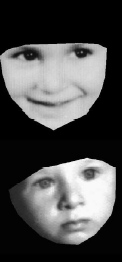
\includegraphics[width=\textwidth]{gandhi/lanitis1.png}
		\caption{оригинал}
	\end{subfigure}
	\begin{subfigure}[t]{0.2\textwidth}
		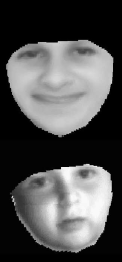
\includegraphics[width=\textwidth]{gandhi/lanitis2.png}
		\caption{имитация возраста}
	\end{subfigure}
	\begin{subfigure}[t]{0.2\textwidth}
		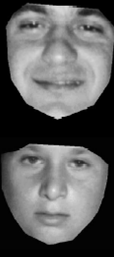
\includegraphics[width=\textwidth]{gandhi/lanitis3.png}
		\caption{реальное лицо}
	\end{subfigure}
	\caption{Результаты из работ Lanitis et al. \cite{lanitis2}}
	\label{fig:lanitis}
\end{figure}

При этом в работах  Lanitis et al. \cite{lanitis} \cite{lanitis2} \cite{lanitis3} для обучения были взяты изображения различного качества с различным освещением, выражением лица, поворотом головы и т.д. Результаты приведены на рис. \ref{fig:lanitis}.

Shan et al. \cite{shan} предложили метод под названием Image-Based Surface Detail Transfer (IBSDT), суть которого в переносе с одного изображения на другое мелких деталей вроде морщин и родинок или больших деталей, таких, как скулы или форма крыльев носа. К сожалению, метод не полностью автоматический, выбор изображения, с которого следует брать детали, должен совершать оператор.

\begin{figure}[t]
	\centering
	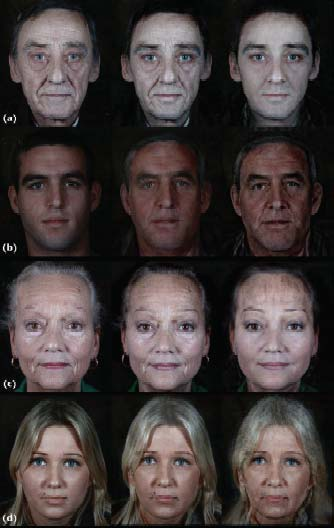
\includegraphics[width=0.3\textwidth]{gandhi/tiddeman.png}
	\caption{Результаты из работы Tiddeman et al. \cite{tiddeman}}
	\label{fig:tiddeman}
\end{figure}

Tiddeman et al. \cite{tiddeman} использовали вейвлеты для описания и преобразования текстуры лица. Имея для каждой возрастной группы лицо-прототип, авторы оценили направления изменений между прототипами для таких не-визуальных параметров, как возраст, пол или раса. Эти изменения затем применялись ко входному лицу. Чтобы результирующее изображение не было слишком гладким (как это бывает во многих методах имитации возраста), прототипы подстраивались под границы, детектируемые на изображении с помощью вейвлетов Габора, основанных на принципах восприятия изображения человеческим глазом (см. рис. \ref{fig:tiddeman}).


\subsubsection{A Method for Automatic Synthesis of Aged Human Facial Images}
Авторы уже упоминавшейся статьи Gandhi \cite{statya_big} описали <<конвейер>> (pipeline), проходя по которому изображение претерпевает множество трансформаций, и лишь затем отдаётся на вход алгоритмам детектирования возраста.

Для имитации изменений возраста авторы предложили воспользоваться методом IBSDT, описанном в статье Shan et al. \cite{shan}. Идея состоит в том, что если наивно перенести изменения между изображениями лиц разных возрастов на новое лицо, то оно будет выглядеть старше (или моложе, в зависимости от того, как считать разницу между изображениями). Например, если на молодое лицо наложить морщины, оно будет выглядеть старше. При этом считается, что лица имеют одинаковые выражения и одинаковое положение всех частей лица. Однако, такая модификация лица не учитывает различный цвет кожи во входном изображении и в обучающих изображениях.

IBSDT исходит из предположения, что изображения лиц соответствуют ламбертовой модели отражения света:
$$
I(P) = \rho(P) l \left \langle \mathbf{n}(P), \mathbf{l}(P) \right \rangle
$$

\begin{figure}[t]
\centering
	\begin{subfigure}[t]{0.2\textwidth}
		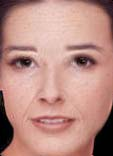
\includegraphics[width=\textwidth]{gandhi/sim1.png}
		\caption{$\sigma = 1$ }
	\end{subfigure}
	\begin{subfigure}[t]{0.2\textwidth}
		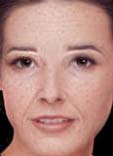
\includegraphics[width=\textwidth]{gandhi/sim2.png}
		\caption{$\sigma = 2$ }
	\end{subfigure}
	\begin{subfigure}[t]{0.2\textwidth}
		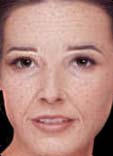
\includegraphics[width=\textwidth]{gandhi/sim3.png}
		\caption{$\sigma = 3$ }
	\end{subfigure}
	\begin{subfigure}[t]{0.2\textwidth}
		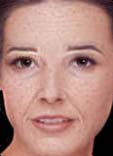
\includegraphics[width=\textwidth]{gandhi/sim4.png}
		\caption{$\sigma = 4$ }
	\end{subfigure}
	\caption{Имитация старения с различными значениями $\sigma$}
	\label{fig:sigmas}
\end{figure}

IBSDT решает проблему переноса нормалей с одного изображения на другое. Из допущения о константности альбедо выводится следующее преобразование изображения:

$$
\widehat{I}_2 = \frac {I_1} {\overline{I}_1} \overline{I}_2
$$

где $ I_1 $ --- изображение, откуда требуется взять нормали, $ I_2 $ --- исходное изображение, на которое требуется перенести нормали, $ \overline{I} $ --- изображение, размытое фильтром Гаусса с некоторым значением параметра $\sigma$ (см. рис. \ref{fig:sigmas}).

Изображения-прототипы были рассчитаны для возрастных групп с разбросом возрастов в 5 лет. Вместо усреднения изображений в группе, которое, по мнению авторов, скрадывает морщины и другие значительные для <<состаривания>> детали, было решено использовать последовательное применение IBSDT к среднему по группе:

$$
\widehat{I} = \frac {I_1} {\overline{I}_1} \cdot \frac {I_2} {\overline{I}_2}  \cdot \ldots \cdot \frac {I_N} {\overline{I}_N} \cdot \overline{I}
$$

где $ \overline{I} $ --- среднее изображение по группе.

Интуиция в этой операции такова: все высокочастотные компоненты отделяются от изображений и усредняются уже на среднем изображении.

Свободный параметр $ \sigma $ при этом оптимизируется с целью уменьшить разницу в возрасте между реальным возрастом группы и предсказанным из полученного прототипа способом, описанным ранее в той же статье.

Таким образом, конвейер по <<состариванию>> (или <<омоложению>>) фотографии выглядит следующим образом:
\begin{enumerate}
	\item выравнивание освещения, позы и выражения лица
	\item детектирование возраста лица
	\item применение к лицу IBSDT для соответствующей целевой возрастной группы
	\item оптимизация параметра $ \sigma $ (цикл по шагам 2 и 3) с целью задетектировать на результирующем лице возраст как можно ближе к целевому
\end{enumerate}

Несколько результирующих изображений, представленных авторами статьи, демонстрируют высокое качество работы алгоритма и схожесть с настоящими фотографиями человека, снятыми в целевом возрасте.

\subsubsection{Illumination-Aware Age Progression}

Со времён выхода статьи Gandhi исследователи не прекращали попыток решить задачу имитации возраста. Суть подхода как правило оставалась той же: найти преобразование лица к нейтральному выражению, определить его текущий возраст и применить к лицу некий набор трансформаций, чтобы сделать его похожим на лицо в целевом возрасте. Однако за это время большой прогресс произошёл в решении подзадач имитации возраста. Так, утвердился в качестве стандарта де-факто метод Виолы-Джонса для поиска лиц \cite{viola_jones}, появились дескрипторы, позволяющие более информативно описать фрагменты изображений (такие, как HOG \cite{hog}, SIFT \cite{sift}, SURF \cite{surf}), более точные точные детекторы ключевых точек лица \cite{jsaragih} \cite{zhu_ramanan} и более эффективные подходы к машинному обучению, такие как deep learning. Появление социальных сетей и веб-поиска по изображениям дало разработчикам алгоритмов доступ к большому количеству изображений практически любых объектов (особенно лиц) с приемлемыми условиями съёмки.

\hyphenation{Re-con-struc-tion Col-lec-tion Me-cha-ni-cal пере-о-све-щён-ных}

Статья Illumination-aware age progression \cite{illumination_aware} вышла в 2014 году и также описывает алгоритм имитации старения лица. Авторы не решают подзадачу оценки возраста, сосредоточившись на имитации возрастных изменений. В статье позаимствованы даже не отдельные методы, а весь конвейер предобработки изображений из статьи Face Reconstruction in the wild от 2011 года \cite{face_wild}. Он включает в себя использование детекторов лиц для их локализации на изображении, поиск ключевых точек лица, гамма-коррекцию и выравнивание позы (но не выражения) лица. В таком обработанном виде изображения поступают на вход алгоритму, описанному в статье.

Обучающую выборку изображений авторы набрали, пользуясь поиском Google по изображениям по запросам вроде <<25 лет>>, <<первый класс>> и т.д., ориенируясь преимущественно на сайты, где был указан возраст сфотографированных людей. Полученные 40 тысяч отобранных вручную изображений были примерно поровну распределены по 14 возрастным группам (0, 1, 2-3, 4-6, 7-9, 10-12, 13-15, 16-24, 25-34, 35-44, 45-56, 57-67, 68-80 и 81-100 лет). 

Для поиска попиксельного соответствия между изображениями внутри каждого кластера авторы использовали собственный алгоритм Collection flow \cite{collection_flow}, который будет описан в следующем разделе. Этот алгоритм позволяет для каждой пары изображений вычислить плотный оптический поток (dense optical flow, здесь и далее под оптическим потоком будет подразумеваться плотный оптический поток), т.е. для каждого пикселя одного изображения найти соответствующий пиксель на другом изображении. Пользуясь таким соответствием, можно искривить лица так, чтобы все они приняли нейтральное выражение и затем посчитать среднее изображение для данного кластера. Однако, авторы предлагают вместо обычных средних изображений использовать средние изображения с освещением, перенесённым из другого изображения, т.е. на каждое входное изображение генерировать серию <<переосвещённых>> (relightable) средних изображений.
Перенос освещения основан на SVD-разложении матрицы, в которую столбец за столбцом (или строка за строкой) помещены изображения лиц. Пусть $ M_j $ - матрица $ f \times p $, где $f$ --- число фотографий в кластере $j$, $p$ --- число пикселей в изображении. Тогда:
$ M_j = U_j D_j V^T_j, $
где $ V^T_j $ --- матрица собственных векторов матрицы ковариации для $ M_j $, $ D_j $ --- диагональная матрица, содержащая собственные числа этих для этих векторов. Таким образом, каждое изображение из $ M_j $ может быть выражено с некоторой точностью через собственные векторы с некоторыми коэффициентами, что является, по сути, реализацией метода главных компонент для векторов, представляющих собой изображения лиц.

Такой подход появился на заре исследований в области распознавания лиц и получил название Eigenfaces. Исследования в этом направлении показали, что первые несколько главных компонент обычно содержат информацию об освещении лица и отдельных его областей (см. рис. \ref{fig:eigenfaces}), следовательно, меняя коэффициенты перед этими компонентами можно имитировать различное освещение.

\begin{figure}[t]
	\centering
	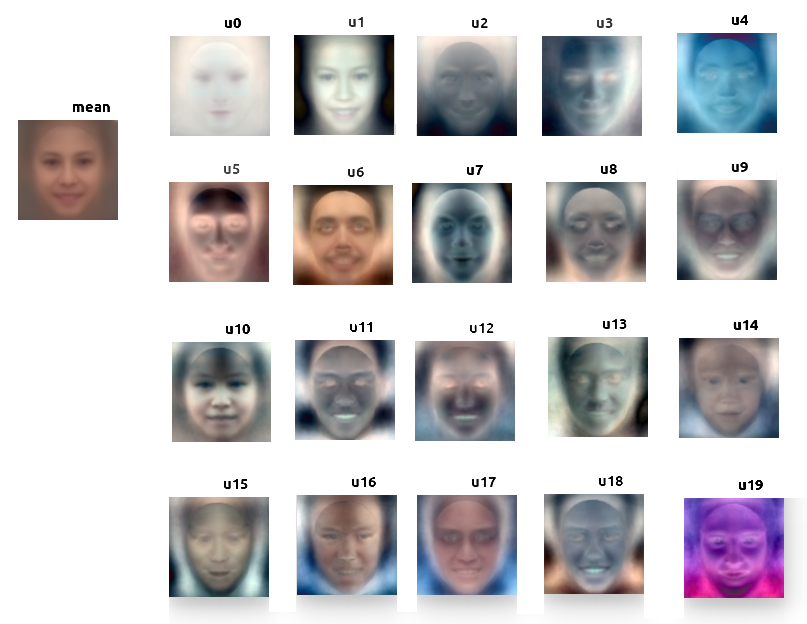
\includegraphics[width=0.5\textwidth]{results/eigenfaces3.png}
	\caption{Eigenfaces: среднее лицо и первые 20 главных компонент}
	\label{fig:eigenfaces}
\end{figure}

Авторы статьи предлагают менять освещение на усреднённом изображении именно таким образом. Ограничив матрицу собственных векторов $ V_j $ до четырёх столбцов, подбираются коэффициенты alpha, приближающие исходное изображение:
$$
\min_{\alpha} || I - \alpha V^T_j || ^2,
$$

где $ I $ --- исходное изображение. Таким образом получаются <<переосвещённые>> средние
 $ A_j^I = \alpha V_j^T $.

Когда изображения внутри кластеров выровнены, требуется найти соответствие (оптический поток) между кластерами. Проблема, однако, заключается в том, что каждый кластер содержит изображения с различным освещением, что можно выразить как различные матрицы $ V_i $ и $ V_j $ для кластеров $ i $ и $j$. Авторы предлагают для поиска плотного оптического потока между кластерами $i$ и $j$ следующую процедуру:

\begin{enumerate}
    \item Пусть $K$ --- число изображений в объединении кластеров $i$ и $j$
    \item Для каждого изображения $ I_k $ из этого объединения пользуясь матрицами $ V_i $ и $ V_j $ вычислить соответственно $ A_i^k $ и $  A_j^k $
    \item Получить два k-канальных изображения $ \textbf{A}_i = \lbrace A_i^k\rbrace_{k=1}^K $, аналогично $ \textbf{A}_j = \lbrace A_j^k \rbrace_{k=1}^K $
    \item Пользуясь сторонним алгоритмом вычислить оптический поток между $ \textbf{A}_i $ и $ \textbf{A}_j$
\end{enumerate}

В результате такого подхода соответствующие каналы двух многоканальных изображений имеют одинаковую освещённость, что нивелирует влияние освещённости на вычисление оптического потока.

В качестве стороннего алгоритма для вычисления оптического потока подойдёт любой алгоритм, способный работать с многоканальными изображениями, например SIFT flow \cite{sift_flow} или SimpleFlow \cite{simple_flow}, которому может работать с изображениями из пикселей любого вида, если для них задана функция дистанции.

Наконец, имитация старения для входного изображения $I$, текущего возраста $s$ и целевого возраста $t$ происходит следующим образом:
\begin{enumerate}
    \item Выровнять изображение $I$ c помощью конвеера из Faces Reconstruction in the Wild \cite{face_wild}
    \item Имитация текстурных изменений
    \begin{enumerate}
        \item Получить <<переосвещённые>> средние $ A^I_s $ и $ A^I_t $
        \item Вычислить оптический поток $ F_{source-input} $ между $ A^I_s $ и $I$, \\
         искривить (warp) $  A^I_s  $ c помощью этого потока, получив $ J_s $
        \item Вычислить оптический поток $ F_{target-input} $ между $ A^I_t $ и $I$, \\
         искривить (warp) $ A^I_t   $ c помощью этого потока, получив $ J_t $
        \item Прибавить к изображению I текстурную разницу: \\
        \mbox{$ I' = I + J_t - J_s $}
    \end{enumerate}

    \item Имитация изменений в потоке
    \begin{enumerate}
        \item Пусть $ F_{target-source} $ --- оптический поток между кластерами s и t, вычисленный заранее
        \item Искривить $I'$ с помощью потока $F_{target-source}$
    \end{enumerate}

    \item Скорректировать пропорции лица: растянуть изображение так, чтобы отношение расстояния между глаз к расстоянию между глазами и ртом соответствовало среднему отношению на кластере $t$
\end{enumerate}

\begin{figure}[t]
\centering
	\begin{subfigure}[t]{0.2\textwidth}
		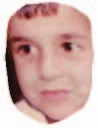
\includegraphics[width=\textwidth]{ilaware_cover1.png}
		\caption{3 года \\ (оригинал)} 
	\end{subfigure}
	\begin{subfigure}[t]{0.2\textwidth}
		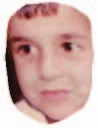
\includegraphics[width=\textwidth]{ilaware_cover2.png}
		\caption{5-7}
	\end{subfigure}
	\begin{subfigure}[t]{0.2\textwidth}
		
\includegraphics[width=\textwidth]{ilaware_cover3.png}
		\caption{14-16}
	\end{subfigure}
	\begin{subfigure}[t]{0.2\textwidth}
		
\includegraphics[width=\textwidth]{ilaware_cover4.png}
		\caption{26-35}
	\end{subfigure}
	\begin{subfigure}[t]{0.2\textwidth}
		
\includegraphics[width=\textwidth]{ilaware_cover5.png}
		\caption{46-57}
	\end{subfigure}
	\begin{subfigure}[t]{0.2\textwidth}
		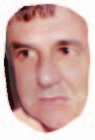
\includegraphics[width=\textwidth]{ilaware_cover6.png}
		\caption{58-68}
	\end{subfigure}		
	\begin{subfigure}[t]{0.2\textwidth}
		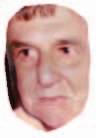
\includegraphics[width=\textwidth]{ilaware_cover7.png}
		\caption{81-100}
	\end{subfigure}
	\caption{Последовательная имитация взросления с использованием Illumination-aware age progression}
	\label{fig:ilaware}
\end{figure}

Результат работы алгоритма приведён на рис. \ref{fig:ilaware}.

Свой алгоритм авторы решили проверить с помощью Amazon Mechanical Turk --- сервиса, который предоставляет труд людей для решения задач, которые компьютеры пока решить не в состоянии. Они давали пользователям три изображения одного и того же человека: фото человека в исходном возрасте, реальное фото человека в целевом возрасте, синтезированное фото в целевом возрасте. Пользователю требовалось определить, какое фото в целевом возрасте является настоящим, были также варианты <<оба фото настоящие>> и <<оба синтезированные>>. Оказалось, что в 37\% случаев пользователи выбирали синтезированное фото, в 41\% --- настоящее. Результат удивил авторов настолько, что они решили оценить, насколько хорошо человек способен сравнивать лица разного возраста. В ещё одном эксперименте пользователям давали две настоящие фотографии одного и того же человека с разницей минимум в пять лет и спрашивали, один ли и тот же человек изображён на фотографиях. По результатам эксперимента оказалось, что люди значительно лучше узнают взрослых спустя разное кол-во лет, чем позврослевших детей. Так, люди узнают детей от 0 до 7 лет с разницей в 10 лет с вероятностью 57\%, с разницей в 20 лет с вероятностью 52\% и с разницей в 50 и более лет с вероятностью 33\%, то есть даже хуже, чем если бы люди бросали монетку. Данное исследование говорит о том, что возможности человека по оценке алгоритмов имитации возраста очень ограничены, и человеческая оценка не всегда может служить объективным показателем качества работы такого рода алгоритмов.

Данная статья широко освещалась в крупных СМИ \cite{wired_age} \cite{telegraph_age} \cite{today_age}. Журналисты подчёркивали реалистичность результатов, сравнивая настоящие изображения человека в целевом возрасте с синтезированными.